\documentclass{article}


\usepackage{arxiv}

\usepackage[utf8]{inputenc} % allow utf-8 input
\usepackage[T1]{fontenc}    % use 8-bit T1 fonts
\usepackage{hyperref}       % hyperlinks
\usepackage{url}            % simple URL typesetting
\usepackage{booktabs}       % professional-quality tables
\usepackage{amsfonts}       % blackboard math symbols
\usepackage{nicefrac}       % compact symbols for 1/2, etc.
\usepackage{microtype}      % microtypography
\usepackage{lipsum}		% Can be removed after putting your text content
\usepackage{amsmath} 
\usepackage{amssymb}
\usepackage{graphicx}
\usepackage{epstopdf}
\usepackage{url}
\usepackage{setspace}
\usepackage{amsthm}
\usepackage{mathrsfs}
\usepackage{enumitem}
\usepackage{parskip}
\usepackage{IEEEtrantools}
\usepackage{mathtools}
\usepackage{tensor}
\usepackage{yfonts}
\usepackage{dsfont}

\usepackage{pgfplots}
\pgfplotsset{compat=1.15}

\usetikzlibrary{arrows}

\definecolor{wwwwww}{rgb}{0.4,0.4,0.4}
\definecolor{wwzzff}{rgb}{0.4,0.6,1}
\definecolor{cqcqcq}{rgb}{0.7529411764705882,0.7529411764705882,0.7529411764705882}

\newtheorem{theorem}{Theorem}[section]
\newtheorem{lemma}[theorem]{Lemma}
\newtheorem*{lemma*}{Lemma}
\newtheorem{prop}[theorem]{Proposition}
\newtheorem{corollary}[theorem]{Corollary}
\newtheorem{defn}[theorem]{Definition\rm}
\newtheorem{conjecture}[theorem]{Conjecture}
\newtheorem{remark}{\it Remark\/}
\newtheorem{example}{Example}
\newtheorem{fact}{Fact}

\newcommand{\st}{\ensuremath{:}}% such that
\newcommand{\ie}{\emph{i.e.} }
\newcommand{\eg}{\emph{e.g.} }
\newcommand{\cf}{\emph{cf.} }
\newcommand{\ra}{\rightarrow}
\newcommand{\la}{\leftarrow}
\newcommand{\lra}{\longrightarrow}
\newcommand{\lla}{\longleftarrow}
\newcommand{\lbracket}{\left(}
\newcommand{\rbracket}{\right)}


\newcommand{\al}{\alpha}
\newcommand{\w}{\omega}
\newcommand{\W}{\Omega}
\newcommand{\m}{\mu}
\newcommand{\n}{\nu}
\newcommand{\e}{\epsilon}
\newcommand{\K}{K\"ahler }
\newcommand{\HK}{hyperk\"ahler }
\newcommand{\into}{\hookrightarrow}
\newcommand{\PP}{\mathbb{P}}
\newcommand{\RR}{\mathbb{R}}
\newcommand{\CC}{\mathbb{C}}
\newcommand{\QQ}{\mathbb{Q}}
\newcommand{\FF}{\mathbb{F}}
\newcommand{\ZZ}{\mathbb{Z}}
\newcommand{\NN}{\mathbb{N}}
\newcommand{\HH}{\mathbb{H}}
\newcommand{\vp}{\varphi}
\newcommand{\mcA}{\mathcal{A}}
\newcommand{\mcE}{\mathcal{E}}
\newcommand{\mcF}{\mathcal{F}}
\newcommand{\mcG}{\mathcal{G}}
\newcommand{\mcH}{\mathcal{H}}
\newcommand{\mcL}{\mathcal{L}}
\newcommand{\mcO}{\mathcal{O}}
\newcommand{\mfg}{\mathfrak{g}}
\newcommand{\mfh}{\mathfrak{h}}
\newcommand{\mft}{\mathfrak{t}}
\newcommand{\mc}[1]{\mathcal{#1}}
\newcommand{\mf}[1]{\mathfrak{#1}}

\newcommand{\dbar}{\bar{\partial}}
\newcommand{\mrr}{\mu_{\mathbb{R}}}
\newcommand{\mcc}{\mu_{\mathbb{C}}}
\newcommand{\prr}{\phi_{\mathbb{R}}}
\newcommand{\pcc}{\phi_{\mathbb{C}}}

\DeclareMathOperator{\Lie}{Lie}
\DeclareMathOperator{\Aut}{Aut}
\DeclareMathOperator{\Tr}{Tr}
\DeclareMathOperator{\Image}{Im}
\DeclareMathOperator{\Ad}{Ad}
\DeclareMathOperator{\Diff}{Diff}
\DeclareMathOperator{\Vect}{Vect}
\DeclareMathOperator{\Sympl}{Sympl}
\DeclareMathOperator{\Span}{Span}
\DeclareMathOperator{\ind}{ind}
\DeclareMathOperator{\Td}{Td}
\DeclareMathOperator{\Ch}{Ch}
\DeclareMathOperator{\Ind}{Ind}
\DeclareMathOperator{\pt}{pt}
\DeclareMathOperator{\rk}{rk}
\DeclareMathOperator{\coker}{coker}
\DeclareMathOperator{\Pf}{Pf}
\DeclareMathOperator{\Vol}{Vol}

\DeclareMathOperator{\GL}{GL}
\DeclareMathOperator{\SO}{SO}
\DeclareMathOperator{\UU}{U}

\newcommand\restr[2]{{% we make the whole thing an ordinary symbol
		\left.\kern-\nulldelimiterspace % automatically resize the bar with \right
		#1 % the function
		\vphantom{\big|} % pretend it's a little taller at normal size
		\right|_{#2} % this is the delimiter
}}

\title{Equivariant Localisation and Fixed-Point Theorems}

\date{12th March 2021}	% Here you can change the date presented in the paper title
%\date{} 					% Or removing it

%\author{
%  David S.~Hippocampus\thanks{Use footnote for providing further
%    information about author (webpage, alternative
%    address)---\emph{not} for acknowledging funding agencies.} \\
%  Department of Computer Science\\
%  Cranberry-Lemon University\\
%  Pittsburgh, PA 15213 \\
%  \texttt{hippo@cs.cranberry-lemon.edu} \\
  %% examples of more authors
%   \And
% Elias D.~Striatum \\
%  Department of Electrical Engineering\\
%  Mount-Sheikh University\\
%  Santa Narimana, Levand \\
%  \texttt{stariate@ee.mount-sheikh.edu} \\
  %% \AND
  %% Coauthor \\
  %% Affiliation \\
  %% Address \\
  %% \texttt{email} \\
  %% \And
  %% Coauthor \\
  %% Affiliation \\
  %% Address \\
  %% \texttt{email} \\
  %% \And
  %% Coauthor \\
  %% Affiliation \\
  %% Address \\
  %% \texttt{email} \\
%}

\begin{document}
\maketitle

\begin{abstract}

Often in mathematics, we are tasked with the problem of evaluating an integral $\int_{M} \w$ over some space $M$. Depending on the form $\w$, this integral can be related to calculating volume, finding topological or enumerative invariants, or integrating characteristic classes. Such computations are often difficult, but two notions can simplify them, which are \emph{symmetry} and \emph{localisation}.

By symmetry, we mean that we have a group $G$ acting on $M$, and by identifying orbits we reduce the problem to that over a smaller space, $M/G$; this comes up in symplectic reduction, gauge theory, and integrable systems. By localisation, this means that we reduce global calculations to local ones; for example, as in the Poincaré-Hopf theorem. Symmetry and localisation synergise together through the Atiyah-Bott-Berline-Vergne fixed-point formula; when we have a smooth manifold $M$ together with the action of a compact, connected Lie group $G$, then the integral on $M$ localises on the fixed-point set of the $G$-action.

In this talk, I want to introduce the equivariant cohomology of a $G$-manifold via the Cartan model - that is, equivariant de Rham theory - before going through some example calculations including the equivariant Riemann-Roch-Hirzebruch, the Duistermaat-Heckman, and the Lefschetz fixed-point theorems.

\end{abstract}

\section{Introduction}

Consider the following geometric sum:

\begin{equation*}
	\begin{split}
		\sum\limits_{k=0}^{10000} q^{k} &= 1 + q + q^{2} + \ldots + q^{10001} \\
		&= \left(\frac{1-q}{1-q}\right)\cdot(1 + q + q^{2} + \ldots + q^{10001}) \\
		&= \frac{1 - q^{10001}}{1 - q} \\
		&= \frac{1}{1 - q} + \frac{1 - q^{10000}}{1 - q^{-1}}.
	\end{split}
\end{equation*}

To evaluate the left-hand side, we need to know the value of each term at the 10001 integral points inside of the closed interval $[0, 10000]$, whereas the right-hand side only needs the two terms to be evaluated. So we can say that this sum \emph{localises} at the end points.

\section{Equivariant Cohomology}

Let $G$ be a compact Lie group acting on a toplogical space $M$. If $G$ acts freely on $M$, then the quotient space $M/G$ is usually as nice as the space $M$ is itself; for instance, if $M$ is a manifold then so is $M/G$.

The idea behind an equivariant cohomology group, $H_{G}^{\ast}(M)$, is that the equivariant cohomology groups of $M$ should just be the cohomology groups of $M/G$:

\begin{equation*}
	H_{G}^{\ast}(M) = H^{\ast}(M/G), \qquad \text{when the action is free.}
\end{equation*}

For example, if $G$ acts on itself by left multiplication, then

\begin{equation*}
	H_{G}^{\ast}(G) = H^{\ast}(\pt).
\end{equation*}

However, if the action is not free, then the space $M/G$ might not behave very nicely from a cohomological point of view. Then the idea is that $H_{G}^{\ast}(M)$ should be the ``correct'' subsitute for $H^{\ast}(M/G)$.

\subsection{Classifying Bundles}

As cohomology is unchanged under homotopy equivalence, our guiding idea is that the equivariant cohomology of $M$ should be the ordinary cohomology of $M^{\ast}/G$, where $M^{\ast}$ is some topological space homotopy equivalent to $M$ and on which $G$ acts freely. The standard way of constructing such a space is to take it to be the product $M^{\ast} = M \times E$, where $E$ is some contractible space on which $G$ acts freely. Then the equivariant cohomology groups of $M$ are defined by the recipe

\begin{equation*}
	H_{G}^{\ast}(M) := H^{\ast}\left( (M \times E)/G \right).
\end{equation*}

Note that if $G$ acts freely on $M$ then the projection

\begin{equation*}
	(M \times E)/G \lra M/G
\end{equation*}

is a fibration with typical fibre $E$. Then as $E$ is contractible, we get that

\begin{equation*}
	H_{G}^{\ast}(M) = H^{\ast}\left( (M \times E)/G \right) = H^{\ast}(M/G),
\end{equation*}

so we arrive at the same situation if $G$ acts freely on $M$.

\subsection{The Cartan Model}

Let $M$ be an $n$-dimensional manifold acted on by a Lie group $G$ with with Lie algebra $\mfg$. A \emph{$G$-equivariant differential form} on $M$ is defined to be a polynomial map $\alpha : \mfg \ra \W(M)$ such that

\begin{equation*}
	\alpha(gX) = g \cdot \alpha(X), \qquad \text{for } g \in G.
\end{equation*}

Let $\CC[\mfg]$ denote the algebra of $\CC$-valued polynomial functions on $\mfg$. Then we can view the tensor product

\begin{equation*}
	\CC[\mfg] \otimes \W(M),
\end{equation*}

as the algebra of polynomial maps from $\mfg$ to $\W$. The group $G$ acts on an element $\alpha \in \CC[\mfg] \otimes \W(M)$ by the formula\footnote{$G$ acts on $\W(M)$ by the induced $G$-action on $M$, and on $\mfg$ by the adjoint action.}

\begin{equation*}
	(g \cdot \alpha)(X) := g \cdot \left( \alpha ( g^{-1} \cdot X )  \right), \qquad \text{for all } g \in G, \text{ and } X \in \mfg.
\end{equation*}

Let $\W^{G}(M) = \left( \CC[\mfg] \otimes \W(M) \right)^{G}$ be the subalgebra of $G$-invariant elements; an element $\alpha \in \W^{G}(M)$ thus satisfies $\alpha(g \cdot X) = g\cdot \alpha(M)$, hence is an equivariant differential form. Equip $\CC[\mfg] \otimes \W(M$ with the following $\ZZ$-grading,

\begin{equation*}
	\deg(P \otimes \alpha) := 2\cdot \deg(P) + \deg(\alpha),
\end{equation*}

for the polynomial $P \in \CC[\mfg]$, and $\alpha \in \W(M)$. Define the \emph{equivariant exterior differential}, or \emph{Cartan differential}, $d_{G}$ by

\begin{equation*}
	(d_{G}\alpha)(X) := (d - \imath_{X_{M}}) \alpha(X),
\end{equation*}

where $d :\W^{k}(M) \ra \W^{k+1}(M)$ is the usual de Rham differential, $X_{M}$ is the fundamental vector field of $X \in \mfg$ on $M$, and $\imath_{X} : \W^{k}(M) \ra \W^{k-1}(M)$ is the contraction of $X$ on a differential form.

\begin{prop}
	The Cartan differential $d_{G}$ is closed on $\W_{G}^{\ast}$, \ie $d_{G}^{2} = 0$.
\end{prop}

\begin{proof}
	
	The derivations $d$ and $\imath_{v}$ in $\W(M)$ are related to the \textbf{Lie derivative} $\mcL$, by means of the \textbf{homotopy formula}:
	
	\begin{equation*}
		\mc{L}(v) := \restr{\frac{d}{dt}}{t = 0} (e^{tv})^{\ast} = d \circ \imath_{v} + \imath_{v} \circ d.
	\end{equation*}
	
	Here $e^{tv}$ is the flow in $M$ after a time $t$ of the velocity field equal to $v$.
	
	Now for $X \in \mfg$, if $X_{M}$ represents the infinitesimal action of $X$ in $M$, then 
	
	[TODO]
	
\end{proof}

\begin{corollary}
	The space of equivariant differential forms $\W_{G}^{\ast}(M) = \left( \CC[\mfg] \otimes \W^{\ast}(M) \right)^{G}$, equipped with the Cartan differential $d_{G}$ forms a complex, called the \textbf{Cartan complex}:
	
	\begin{equation*}
		\left( \W_{G}^{\ast}(M), d_{G} \right) = \left( (\CC[\mfg] \otimes \W^{\ast}(M)   )^{G}, d_{G} \right).
	\end{equation*}

\end{corollary}

\begin{defn}
	The \textbf{equivariant cohomology} $H_{G}^{\ast}(M)$ of $M$ is the cohomology of the Cartan complex, $(\W_{G}^{\ast}(M), d_{G})$.
\end{defn}

\subsection{Characteristic Classes}

Let $G$ and $T$ be compact, connected Lie groups.

An ordinary characteristic class for a principal $G$-bundle on an $n$-dimensional manifold $M$ is $[p(F_{A})] \in H^{2n}(M)$, for a $G$ -invariant degree $n$ polynomial $p \in \RR[\mfg]^{G}$. here $F_{A}$ is the curvature of any connection $A$ on the $G$-bundle.

To get a $T$-equivariant characteristic class for a principal $G$-bundle associated to a $G$-invariant, degree $n$ polynomial $p \in \RR[\mfg]^{G}$, we take $[p(F_{A, T})] \in H_{T}^{2n}(M)$, where now $F_{A,T}$ is the $T$-equivariant curvature of any $T$-equivariant connection $A$ on the $G$-bundle.

Restricted to the $T$-fixed points $M^{T}$ of $M$, the $T$-equivariant characteristic class associated to a polynomial $p \in \RR[\mfg]^{G}$ is

\begin{equation*}
	p(F_{A} + \e^{a}\rho(T_{a})).
\end{equation*}

TODO: EXPLAIN WHAT $\e^{a}$, etc. ARE!

In particular, when $V$ is a representation of $G$ and $p$ is the Chern character of the vector bundle $V$, then, if $M$ is a point, the equivariant Chern characters are just the ordinary characters of the space $V$ as a $G$-module.

\subsection{The Euler Class}

Here, let $G = \SO(2n)$ which preserves the Riemannian metric on an oriented real vector space $V$ of dimension $\dim_{\RR}(V) = 2n$.

\begin{defn}
	Consider the following adjoint-invariant polynomial,
	
	\begin{equation*}
		\Pf : \mf{so}(2n;\RR) \lra \RR,
	\end{equation*}

	of degree $n$ on the Lie algebra $\mf{so}(2n;\RR)$, called the \textbf{Pfaffian}.
	
	The case that we shall be interested in is when we have the $(2n \times 2n)$-antisymmetric matrix,
	
	\begin{equation*}
		\Pf
		\begin{pmatrix}
			0 & \lambda_{1} & \dots & \dots & 0 & 0 \\
			-\lambda_{1} & 0 & \dots & \dots & 0 & 0 \\
			\vdots & \vdots & \ddots & \vdots & \vdots & \vdots \\
			\vdots & \vdots & \dots & \ddots & \vdots & \vdots \\
			0 & 0 & \dots & \dots & 0 & \lambda_{n} \\
			0 & 0 & \dots & \dots & -\lambda_{n} & 0			
		\end{pmatrix}
		= \lambda_{1}\cdot\ldots \cdot \lambda_{n}.
	\end{equation*}
	
\end{defn}

\begin{defn}
	
	Let $P \ra M$ be an $\SO(2n;\RR)$-principal bundle over $M$. The \textbf{Euler characteristic class} of $P$, $e(P)$, is given by
	
	\begin{equation*}
		e(P) := [\Pf(F)] \in H^{2n}(M; \ZZ).
	\end{equation*}

\end{defn}

\begin{example}
	If $M$ is an oriented, $2n$-dimensional real manifold, then the \textbf{Euler characteristic} is given by

	\begin{equation*}
		e(M) = \int_{M} e(TM) = \int_{M} \Pf(R_{\nabla}),
	\end{equation*}

	where $R_{\nabla}$ is the curvature form of the tangent bundle $TM$, equipped with the Levi-Civita connection.
\end{example}

To upgrade the Euler characteristic class $e$ to a $T$-equivariant one $e_{T}$, where $T$ is a torus acting on a manifold $M$ with isolated fixed-point set $M^{T}$, we need to investigate the polynomial

\begin{equation*}
	\Pf(F_{A} + \e^{a}\rho(T_{a})).
\end{equation*}

For simplicity, let $T = S^{1}$. Then, for a point $p \in M^{S^{1}}$, the $S^{1}$-action on $T_{p}M$ gives rise to an $S^{1}$-representation,

\begin{equation*}
	\rho : S^{1} \lra \GL(T_{m}M); \qquad g \longmapsto l_{g, \ast},
\end{equation*}

where $l_{g, \ast} : T_{p}M \ra T_{g\cdot p}M = T_{p}M$ is the differential of the action of $g \in S^{1}$ on $T_{m}M$.

As $p$ is isolated, $\rho$ decomposes into a direct sum of $2$-dimensional irreducible representations,

\begin{equation*}
	T_{p}M \cong L^{m_{1}} \oplus \ldots \oplus L^{m_{n}}.
\end{equation*}

Here, $L^{m} : S^{1} \ra \GL(2;\RR)$ is a representation of $S^{1}$ as $m$-fold rotations in $\RR^{2}$,

\begin{equation*}
	L^{m} : g \longmapsto l_{g,\ast}; \qquad
	L^{m}(e^{it}) =
	\begin{bmatrix}
		-m\sin(mt) & -m\cos(mt) \\
		m\cos(mt) & -m\sin(mt)
	\end{bmatrix}.
\end{equation*}

\subsection{Chern Classes}

Now let $G = \UU(n)$, then $\mfg = \mf{u}(n)$ can be identified with the space of matrices of the form $iA$, where $A = A^{T}$. Define the polynomial $c_{k}$, of degree $k$ in $A$ to be the coefficient of $(-1)^{k}\lambda^{n-k}$ in the characteristic polynomial of $A$:

\begin{equation*}
	\det(\lambda - A) = \lambda^{n} - c_{1}(A)\lambda^{n-1} + \ldots + (-1)^{n}c_{n}(A).
\end{equation*}

In particular, $c_{1}(A) = \Tr(A)$ and $c_{n}(A) = \det(A)$. These polynomials are clearly adjoint invariant, thus the characteristic polynomial is.

The characteristic classes corresponding to the $c_{i}$ for a complex vector bundle are called its \textbf{Chern classes}.

\begin{remark}
	If we consider a complex vector bundle $V_{\CC}$ of $\dim_{\CC}(V) = n$ then, by forgetting the complex structure on $V_{\CC}$, we get an oriented real vector bundle $V_{\RR}$ of real dimension $\dim_{\RR}(V) = 2n$.
	
	By this correspondence, the Euler class $e(V)$ and the top Chern class $c_{n}(V)$ of $V$ are related by
	
	\begin{equation*}
		e(V_{\RR}) = c_{n}(V_{\CC}).
	\end{equation*}
	
\end{remark}

\subsection{Equivariant Characteristic Classes}

\begin{defn}
	A $G$\textbf{-equivariant vector bundle} of a $G$-manifold $M$ is a vector bundle $V \ra M$ with an action of $G$ on the total space $V$ covering the action of $G$ on $M$.
\end{defn}

\begin{defn}
	Let $(M, \w)$ be a symplectic manifold, and suppose that a torus $T$ acts on $M$ preserving $\w$. The action is \textbf{Hamiltonian} if there exists a \textbf{moment map} $\mu : M \ra \mft^{\ast}$, whuch satisfies
	
	\begin{equation*}
		\imath_{\xi_{M}}\w = d\langle \mu,\, \xi \rangle, \quad \text{for all } \xi \in \mft.
	\end{equation*}

	Here, $\xi_{M}$ is the induced vector field on $M$.
\end{defn}

\begin{prop}
	Let $(M, \w, \mu)$ be a symplectic manifold with a Hamiltonian action of a torus $T$ and associated moment map $\mu : M \ra \mft^{\ast}$. Set
	
	\begin{equation*}
		\tilde{\w} := \w + \mu.
	\end{equation*}
	
	Then $\tilde{\w}$ is a $T$-equivariantly closed two-form.
\end{prop}

\begin{proof}
	For $\tilde{\w}$ to be equivariantly closed under $d_{T}$, we have
	
	\begin{equation*}
		d_{T}\tilde{\w} = 0 \iff (d - \imath_{\xi})(\w + \mu^{\xi}) = d\w - \imath_{\xi}\w + d\mu^{\xi} - \imath_{\xi}\mu^{\xi} = -\imath_{\xi}\w + d\mu^{\xi} = 0 \iff \imath_{\xi}\w = d\mu^{\xi}.
	\end{equation*}
\end{proof}

So given an ordinary characteristic class $[\w] \in H^{2}(M)$ and a moment map $\mu : M \ra \mfg^{\ast}$, we can elevate it to an equivariant characteristic class by the substitution

\begin{equation*}
		H^{2}(M) \ni [\w] \longmapsto [\w_{G}] = [\w + \mu] \in H_{G}^{2}(M).
\end{equation*}

\newpage

\begin{prop}
	If $E$ is a complex vector bundle with a $T$-action and $E \cong \bigoplus_{j} \mcL_{j}$, where $\mcL_{j}$ are complex line bundles with $T$-action given by weights $\lambda_{j} : T \ra U(1)$, then the equivariant Euler class of $E$ is
	
	\begin{equation*}
		e^{T}(E) = \prod\limits_{j} c_{1}^{T}(\mcL_{j}).
	\end{equation*}
	In the Cartan model, this is represented by
	\begin{equation*}
		e^{T}(E)(\xi) = \prod\limits_{j} (F_{j} - \lambda_{j})(\xi).
	\end{equation*}
\end{prop}

\begin{example}
	If $T$ acts on $M$ and $F$ is a component of $M^{T}$, then the normal bundle $\nu_{F}$ is a $T$-equivariant bundle over $V$. Assume that $\nu_{F}$ decomposes equivariantly as $\nu_{F} \cong \bigoplus_{j} \nu_{F, j}$ with weights $\lambda_{F, j} \in \mft^{\ast}$. Then the equivariant Euler class $e^{T}(\nu_{F})$ is
	\begin{equation*}
		e^{T}(\nu_{F}) = \prod\limits_{j} \left( c_{1}(\nu_{F,j}) + \beta_{F,j} \right).
	\end{equation*}

	When the fixed-point set $M^{T}$ consists of isolated fixed-points then, for $p \in M^{T}$,
	
	\begin{equation*}
		e^{T}(\nu_{p})
	\end{equation*}

\end{example}



\newpage










\newpage

\section{Equivariant Localisation}






\subsection{The Berline-Vergne-Atiyah-Bott Fixed Point Theorem}

When a manifold has a torus action, the equivariant localisation formula is a powerful tool for doing calculations in \textbf{ordinary} cohomology, despite being formulated in \textbf{equivariant} cohomology.

\begin{theorem}[\textbf{Atiyah-Bott, Berline-Vergne Theorem}]
	Suppose an $n$-dimensional torus $T$ acts on a compact oriented manifold $M$ with fixed-point set $F := M^{T}$. If $\phi$ is an equivariant closed form on $M$ and $i_{F}: F \hookrightarrow M$ is the inclusion map, then
	\begin{equation*}
		\int_{M} \phi = \sum\limits_{F \subseteq M^{T}} \int_{F} \frac{i_{F}^{\ast} \phi}{e^{T}(\nu_{F})},
	\end{equation*}
	as elements of $H_{T}^{\ast}(\pt) = \RR[u_{1}, \ldots, u_{n}]$. Here, $\nu_{F}$ is the normal bundle of $F$ in $M$, and $e^{T}$ is the $T$-equivariant Euler class.
\end{theorem}

In the case when the fixed-point set $M^{T} = \{p_{i}\}$ consists of isolated fixed-points, the localisation theorem simplifies greatly:

\begin{theorem}
	With the above hypotheses, if $M^{T}$ consists of isolated fixed-points, then:
	\begin{equation*}
		\int_{M} \phi = \sum\limits_{p \in M^{T}} \frac{\phi(p)}{\prod_{i} \lambda_{p, i}}.
	\end{equation*}
\end{theorem}


\section{Examples}


\subsection{The Index and Hirzebruch-Riemann Roch Theorems}

\begin{theorem}[\textbf{Hirzebruch-Riemann-Roch, (HRR)}]
	Let $\mcL \ra M$ a holomorphic line bundle over a \textbf{complex projective algebraic variety} $M$. Then the Euler characteristic, $\chi(M; \mcL)$, is equal to the characteristic number
	\begin{equation*}
		\chi(M; \mcL) =	\int_{M} e^{c_{1}(\mcL)}\, \Td(TM).
	\end{equation*}
	Here, $c_{1}(\mcL)$ is the \emph{1st Chern class} of $\mcL$, and $\Td(M)$ is the \emph{Todd class} of the complex vector bundle $TM \ra M$.
\end{theorem}

\begin{defn}
	The \textbf{Todd class} $\Td(TM)$ of a complex tangent bundle $(TM, J)$ is
	\begin{equation*}
		\Td(TM) := \prod_{j = 1}^{n} \frac{c_{1}}{1 + e^{-c_{1}}},
	\end{equation*}
	where $c_{1} := c_{1}(TM)$ is the 1st Chern class of the tangent bundle.
\end{defn}

\begin{example}
	Let $M = \CC\PP^{1}$ and $\mcL = \mcO(k)$. Then $c_{1}(\mcL) = kH$, where $H$ generates $H^{2}(\CC\PP^{1}; \ZZ)$. The Chern character of $\mcL$ is
	\begin{equation*}
		e^{c_{1}(\mcL)} = 1 + kH.
	\end{equation*}
	The tangent bundle $TM$ is a line bundle with 1st Chern class $c_{1}(TM) = 2H$, so its Todd class is
	\begin{equation*}
		\Td(c_{1}(TM)) = \frac{c_{1}(TM)}{1 + e^{-c_{1}(TM)}} = 1 + \frac{1}{2}c_{1}(TM) = 1 + H.
	\end{equation*}
	Thus, the Riemann-Roch integral is
	\begin{equation*}
		\int_{M} (1 + kH)(1 + H) = \int_{M} (k+1)H + 1 = k+1.
	\end{equation*}
	In particular, if $k = 10000$, then we get $\chi(\CC\PP^{1}; \mcL) = 10001$, which we saw at the start of this talk.
\end{example}

\begin{remark}
	The sections of $\mcL$ can be identified with degree $k$ polynomials in the two coordinate variables of $\CC\PP^{1}$, and hence the space of sections has dimension $k+1$. The higher cohomology spaces vanish: $H^{j}(\CC\PP^{1}; \mcL) = 0$ if $j \geq 1$ by Kodaira vanishing.
\end{remark}

This integral formula was originally proven for complex projective algebraic varieties by Hirzebruch, but the Atiyah-Singer index theorem generalises it to include complex analytic manifolds by the following argument:

The characteristic number $\chi(M; \mcL)$ also equals
\begin{equation*}
	\chi(M; \mcL) = \sum (-1)^{k} \dim H^{k}(M; \mcL).
\end{equation*}
Provided that $M$ has a Hermitian structure and hence metric, then this metric gives rise to an inner-product on the vector bundles $\Lambda^{0,k} = \Lambda^{0,k}TM$. Moreover, provided $\mcL$ also has a Hermitian structure, then there are Hermitian inner-products on the vector bundles $\mcL \otimes \Lambda^{0,k}$ also. These Hermitian products and the volume form give rise to differential operators,
	\begin{equation*}
		\bar{\partial}^{\ast} : \W^{0,k}(M; \mcL) \lra \W^{0,k-1}(M; \mcL),
	\end{equation*}
as the product gives rise to an adjoint to the Dolbeault operator, $\bar{\partial}$. By Hodge theory, one can show that
	\begin{equation*}
		\ind(\bar{\partial}) := \ker( \bar{\partial} + \bar{\partial}^{\ast} ) - \coker( \bar{\partial} + \bar{\partial}^{\ast} ) =  \sum (-1)^{k} \dim H^{k}(M; \mcL),
	\end{equation*}
as virtual vector spaces.

\subsection{The Equivariant Index Theorem}

Suppose now that in addition to the hypotheses above, we now have a bundle automorphism $\gamma$ of $\mcL$, which leaves all the given structures in variant. Then it induces an operator on $\Lambda^{0,\ast}$ which commutes with $\bar{\partial}$. Hence if $\gamma$ comes from a representation of a $G$-action, we get a \textbf{virtual representation} on $\Ind(\bar{\partial})$, by lifting the $G$-action to the sections of $\mcL$. Letting $\chi$ denote the character of this representation and letting $G = T$ be a torus, then we have:

\begin{theorem}[\textbf{The Equivariant Index Formula}]
	\begin{equation*}
		\Ind(\bar{\partial}; \mcL, T)(\xi) = \chi(e^{it}) = \int_{M} e^{c_{1}^{T}(\mcL)(\xi)} \Td^{T}(TM)(\xi), \qquad t \in \mft.
	\end{equation*}
\end{theorem}

\begin{example}
	In the case when the set $M^{T}$ fixed points is isolated, we obtain the \textbf{equivariant Lefschetz fixed-point formula}:
	\begin{equation*}
		\Ind(\bar{\partial}; \mcL)(t) = \sum\limits_{p \in M^{T}} \frac{\Tr_{\mcL_{p}}(t)}{\det_{T_{p}^{1,0}}(1 - t^{-1})}.
	\end{equation*}
\end{example}

\begin{fact}
	When the $T$-action on a symplectic manifold $(M, \w)$ is Hamiltonian with moment map $\mu : M \ra \mft^{\ast}$, the image of $\mu$ is a convex polytope, whose vertices are the images of the fixed-points of the $T$-action. The isotropy weights at each fixed-point $p \in M^{T}$ are given by the primitive edge vectors $\alpha_{p,j} \in \mft^{\ast}$, $j = 1\ldots, \dim_{\CC} M$.
	
	Moreover for symplectic toric manifolds, the weights of the $T$ action on $H^{0}(M, \mcL)$ are given by the lattice points in the moment polytope $\mu(M)$. In particular, a weight of the $T$-representation appears only if it is contained in the image of the moment map, and has multiplicity one.
\end{fact}

\begin{example}
	Let $M = \CC\PP^{1}$ and $G = U^{1}$ act on $M$ as
	\begin{equation*}
		t \cdot [z_{0}: z_{1}] = [z_{0} : tz_{1}],
	\end{equation*}

	and let $\mcL = \mcO(n)$ be a complex line bundle of degree $n$ over $\CC\PP^{1}$. Then the moment map for this action $\mu : \CC\PP^{1} \ra \RR^{\ast}$ is
	\begin{equation*}
		\mu([z_{0}:z_{1}]) = n\cdot\frac{|z_{1}|^{2}}{|z_{0}|^{2} + |z_{1}|^{2}},
	\end{equation*}
	with image $\mu(\CC\PP^{1}) = [0, n]$. The primitive edge vectors for the two fixed-points are
	\begin{equation*}
		\alpha_{[1:0]} = +1, \qquad \alpha_{[0:1]} = -1,
	\end{equation*}
	and the images of $\mu$ at these two fixed-points are
	\begin{equation*}
		 \mu([1:0]) = 0, \qquad \mu([0:1]) = n,
	\end{equation*}
	giving us the weights on the fibres of $\mc{O}(n)$ at these two points. Thus
	
	\begin{equation*}
		\Ind(\bar{\partial}; \mcL, \CC\PP^{1})(t) = \frac{1}{1 - t} + \frac{t^{n}}{1 - t^{-1}} = \sum_{k = 0}^{n}t^{n}, \qquad n \geq 0.
	\end{equation*}

\end{example}

\begin{example}
	Now for $M =\CC\PP^{2}$ with $T^{2}$-action
	\begin{equation*}
		(t_{1},t_{2}) \cdot [z_{0} : z_{1} : z_{2}] = [z_{0} : t_{1}z_{1} : t_{2}z_{2}],
	\end{equation*}
	and moment map $\mu : M \ra \RR^{2}$ given by
	\begin{equation*}
		\mu([z_{0}: z_{1} : z_{2}]) = n\cdot \left( \frac{|z_{1}|^{2}}{\|z\|^{2}}, \frac{|z_{2}|^{2}}{\|z\|^{2}} \right),
	\end{equation*}
	for the bundle $\mcL = \mcO(n)$, so its moment map image is the dilated $2$-simplex,
	\begin{equation*}
		\mu(M) = n\cdot \Delta = \{ (x,y) \in \RR^{2}_{\geq 0} \st x + y \leq n \}.
	\end{equation*}
	As before, we can read off the combinatorial data required from the polytope:
	\begin{alignat*}{3}
		&\mu([1:0:0]) = p_{0} = (0,0), \qquad && \alpha_{1,1} = (1,0), \qquad	&& \alpha_{1,2} = (0,1), \\
		&\mu([0:1:0]) = p_{1} = (n,0), \qquad&& \alpha_{2,1} = (-1,1), \qquad && \alpha_{2,2} = (-1,0), \\
		&\mu([0:0:1]) = p_{2} = (0,n), \qquad && \alpha_{3,1} = (0,-1), \qquad && \alpha_{3,2} = (1,-1).
	\end{alignat*}
	
\begin{center}
	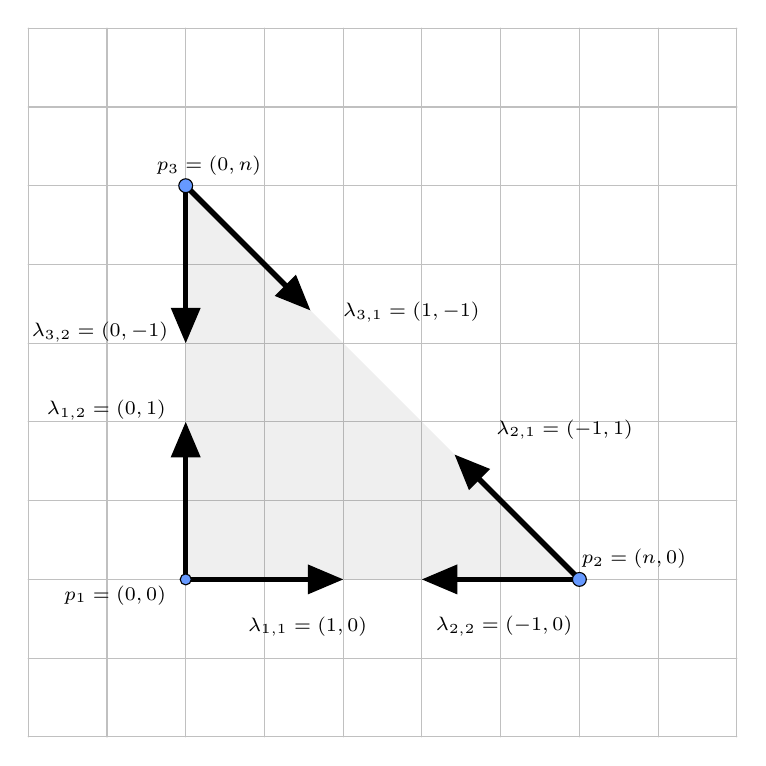
\begin{tikzpicture}[line cap=round,line join=round,>=triangle 45,x=1cm,y=1cm]
		\draw [color=cqcqcq,, xstep=1cm,ystep=1cm] (-2,-2) grid (7,7);
		\clip(-2,-2) rectangle (7,7);
		\fill[line width=2pt,color=wwwwww,fill=wwwwww,fill opacity=0.1] (0,0) -- (0,5) -- (5,0) -- cycle;
		\draw [->,line width=2pt] (0,5) -- (0,3);
		\draw [->,line width=2pt] (0,0) -- (0,2);
		\draw [->,line width=2pt] (0,0) -- (2,0);
		\draw [->,line width=2pt] (5,0) -- (3,0);
		\draw [->,line width=2pt] (5,0) -- (3.415476370307829,1.5845236296921712);
		\draw [->,line width=2pt] (0,5) -- (1.5823813554983261,3.417618644501674);
		\begin{scriptsize}
			\draw [fill=wwzzff] (0,0) circle (2pt);
			\draw[color=black] (-0.8958350907930224,-0.2) node {$p_{1} = (0,0)$};
			\draw [fill=wwzzff] (0,5) circle (2.5pt);
			\draw[color=black] (0.2958350907930224,5.256479409233972) node {$p_{3} = (0,n)$};
			\draw [fill=wwzzff] (5,0) circle (2.5pt);
			\draw[color=black] (5.691427001254021,0.2608874987729722) node {$p_{2} = (n,0)$};
			\draw[color=black] (-1.08970629837108796,3.140958885538797) node {$\lambda_{3,2} = (0,-1)$};
			\draw[color=black] (-1.007295486298057659,2.146028783878926) node {$\lambda_{1,2} = (0,1)$};
			\draw[color=black] (1.547598921978901,-0.60026138335475616) node {$\lambda_{1,1} = (1,0)$};
			\draw[color=black] (4.042529023638772,-0.59113437560196733) node {$\lambda_{2,2} = (-1,0)$};
			\draw[color=black] (4.812282146809777,1.9035243222060619) node {$\lambda_{2,1} = (-1,1)$};
			\draw[color=black] (2.8657205757242529,3.395588570295304) node {$\lambda_{3,1} = (1,-1)$};
		\end{scriptsize}
	\end{tikzpicture}
\end{center}

Putting this all together into the index formula, we get
\begin{equation*}
	\begin{split}
		\Ind(\bar{\partial}, M, \mcO(n))(t_{1},t_{2}) &= \frac{1}{1 - t_{1}t_{2}} + \frac{t_{1}^{n}}{(1 - t_{1}^{-1})(1 - t_{1}^{-1}t_{2})} + \frac{t_{2}^{n}}{(1 - t_{2}^{-1})(1 - t_{1}t_{2}^{-1})} \\
		&= \sum\limits_{\substack{0 \leq n_{1}, n_{2} \\ n_{1} + n_{2} \leq n}} t_{1}^{n_{1}}t_{2}^{n_{2}}.
	\end{split}
\end{equation*}
The last equality can be determined by expanding each rational polynomial expression into its Laurent series, then calculating the coefficients by the residue theorem.

[TODO]: Jupyter notebook.

\subsection{Duistermaat-Heckman and the Stationary Phase Approximation}

In physics, many integrals are of the form
\begin{equation*}
	\int_{M} e^{itf}d\mu,
\end{equation*}
where $M$ is a compact oriented $n$-manifold, $f$ is a function, and $\mu$ is an $n$-form on $M$. Such an integral is called an \textbf{oscillatory integral}. Examples of situations in which they come up include Fourier transformations, path integrals, etc.

The method of stationary phase gives an approximation to such an oscillatory integral, based on the critical points of the function $f$; it is at these points that $f$ does not change fast enough to cancel out its other values, contributing to the value to the integral. However in the case that $(M, \w)$ is a symplectic manifold and $S^{1}$ acts symplectically on $M$ with isolated fixed-point set $F = M^{S^{1}}$, the equivariant localisation formula gives an \textbf{exact} value:

\begin{theorem}[\textbf{Duistermaat-Heckman}]
	Consider an $n$-dimensional manifold $(M, \w, \mu)$ with Hamiltonian $S^{1}$-action and moment map $\mu : M \ra \RR$. Then, for any $\hbar \in \CC$:
	\begin{equation*}
		\int_{M} e^{\hbar \mu} \frac{\w^{n}}{n!} \equiv \int_{M} e^{\w + \hbar \mu} = \left(\frac{-1}{\hbar}\right)^{n} \sum_{p\in F} \frac{e^{\hbar \mu(p)}}{\prod_{j=1}^{n}\alpha_{p,j}(p)},
	\end{equation*}
	where the $\alpha_{p,j}$, $j = 1, \ldots, n$, are the isotropy weights for the $S^{1}$-action at the fixed point $p$.
\end{theorem}

\begin{example}
	Let $S^{1}$ act on $(S^{2}, \w)$ by rotating the sphere around its $z$-axis in a counter-clockwise orientation (when viewed from above) with period $1$ (or with speed $2\pi$). 
	
	[TODO]: Refresh remind yourself of spherical coordinates....

\end{example}

\begin{remark}
	Expanding out the Duistermaat-Heckman formula in terms of $\hbar$, we get:
	\begin{equation*}
		\begin{split}
			\int_{M} \cdot \frac{\w^{n}}{n!}\left( 1 + \hbar \mu + \ldots \right) = \left(\frac{-1}{\hbar}\right)^{n} \sum\limits_{p\in F} \left( 1 + \hbar\mu(p) + \ldots + \frac{\hbar^{n}\mu(p)^{n}}{n!} + \ldots \right) / \prod_{j = 1}^{n} \alpha_{p,j}.
		\end{split}
	\end{equation*}
	Of special interest is the degree-$0$ term which, after cancelling factors, gets us a formula for the volume of $M$ in terms of its fixed-point data:
	
	\begin{equation*}
		\Vol(M) = \int_{M} \w^{n} = (-1)^{n} \sum\limits_{p\in F} \frac{\mu(p)^{n}}{\prod_{j = 1}^{n}\alpha_{p,j}}.
	\end{equation*}
\end{remark}




\end{example}









\bibliographystyle{unsrt}  
%\bibliography{references}  %%% Remove comment to use the external .bib file (using bibtex).
%%% and comment out the ``thebibliography'' section.


%%% Comment out this section when you \bibliography{references} is enabled.

\end{document}
